% Created by tikzDevice version 0.12 on 2019-07-15 12:54:16
% !TEX encoding = UTF-8 Unicode
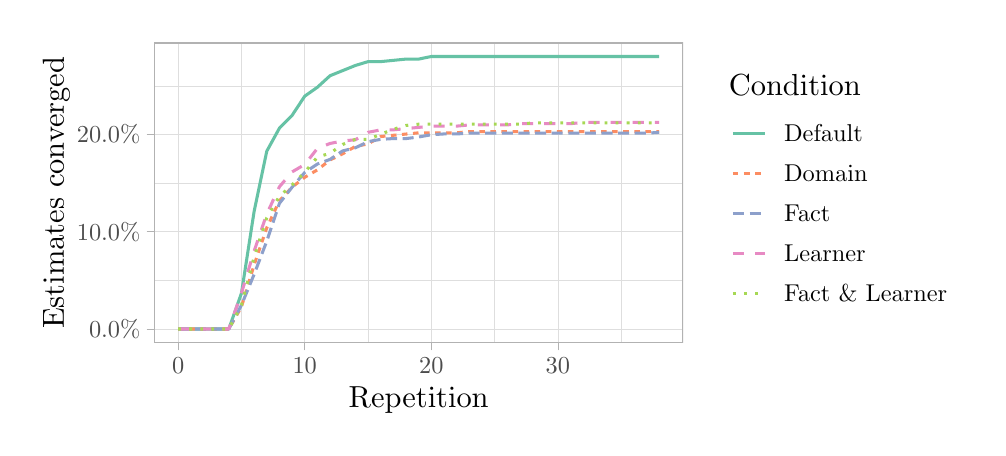
\begin{tikzpicture}[x=1pt,y=1pt]
\definecolor{fillColor}{RGB}{255,255,255}
\path[use as bounding box,fill=fillColor,fill opacity=0.00] (0,0) rectangle (343.28,144.54);
\begin{scope}
\path[clip] (  0.00,  0.00) rectangle (343.28,144.54);
\definecolor{drawColor}{RGB}{255,255,255}
\definecolor{fillColor}{RGB}{255,255,255}

\path[draw=drawColor,line width= 0.6pt,line join=round,line cap=round,fill=fillColor] (  0.00, -0.00) rectangle (343.28,144.54);
\end{scope}
\begin{scope}
\path[clip] ( 45.69, 30.72) rectangle (236.88,139.04);
\definecolor{fillColor}{RGB}{255,255,255}

\path[fill=fillColor] ( 45.69, 30.72) rectangle (236.88,139.04);
\definecolor{drawColor}{gray}{0.87}

\path[draw=drawColor,line width= 0.1pt,line join=round] ( 45.69, 53.22) --
	(236.88, 53.22);

\path[draw=drawColor,line width= 0.1pt,line join=round] ( 45.69, 88.35) --
	(236.88, 88.35);

\path[draw=drawColor,line width= 0.1pt,line join=round] ( 45.69,123.48) --
	(236.88,123.48);

\path[draw=drawColor,line width= 0.1pt,line join=round] ( 77.25, 30.72) --
	( 77.25,139.04);

\path[draw=drawColor,line width= 0.1pt,line join=round] (122.99, 30.72) --
	(122.99,139.04);

\path[draw=drawColor,line width= 0.1pt,line join=round] (168.73, 30.72) --
	(168.73,139.04);

\path[draw=drawColor,line width= 0.1pt,line join=round] (214.47, 30.72) --
	(214.47,139.04);

\path[draw=drawColor,line width= 0.3pt,line join=round] ( 45.69, 35.65) --
	(236.88, 35.65);

\path[draw=drawColor,line width= 0.3pt,line join=round] ( 45.69, 70.78) --
	(236.88, 70.78);

\path[draw=drawColor,line width= 0.3pt,line join=round] ( 45.69,105.92) --
	(236.88,105.92);

\path[draw=drawColor,line width= 0.3pt,line join=round] ( 54.38, 30.72) --
	( 54.38,139.04);

\path[draw=drawColor,line width= 0.3pt,line join=round] (100.12, 30.72) --
	(100.12,139.04);

\path[draw=drawColor,line width= 0.3pt,line join=round] (145.86, 30.72) --
	(145.86,139.04);

\path[draw=drawColor,line width= 0.3pt,line join=round] (191.60, 30.72) --
	(191.60,139.04);
\definecolor{drawColor}{RGB}{102,194,165}

\path[draw=drawColor,line width= 1.1pt,line join=round] ( 54.38, 35.65) --
	( 58.96, 35.65) --
	( 63.53, 35.65) --
	( 68.10, 35.65) --
	( 72.68, 35.65) --
	( 77.25, 48.59) --
	( 81.83, 78.18) --
	( 86.40, 99.91) --
	( 90.97,108.23) --
	( 95.55,112.85) --
	(100.12,119.79) --
	(104.70,123.02) --
	(109.27,127.18) --
	(113.84,129.03) --
	(118.42,130.88) --
	(122.99,132.27) --
	(127.57,132.27) --
	(132.14,132.73) --
	(136.71,133.19) --
	(141.29,133.19) --
	(145.86,134.12) --
	(150.44,134.12) --
	(155.01,134.12) --
	(159.58,134.12) --
	(164.16,134.12) --
	(168.73,134.12) --
	(173.30,134.12) --
	(177.88,134.12) --
	(182.45,134.12) --
	(187.03,134.12) --
	(191.60,134.12) --
	(196.17,134.12) --
	(200.75,134.12) --
	(205.32,134.12) --
	(209.90,134.12) --
	(214.47,134.12) --
	(219.04,134.12) --
	(223.62,134.12) --
	(228.19,134.12);
\definecolor{drawColor}{RGB}{252,141,98}

\path[draw=drawColor,line width= 1.1pt,dash pattern=on 2pt off 2pt ,line join=round] ( 54.38, 35.65) --
	( 58.96, 35.65) --
	( 63.53, 35.65) --
	( 68.10, 35.65) --
	( 72.68, 35.65) --
	( 77.25, 43.67) --
	( 81.83, 58.83) --
	( 86.40, 72.21) --
	( 90.97, 82.02) --
	( 95.55, 86.92) --
	(100.12, 90.49) --
	(104.70, 93.16) --
	(109.27, 96.73) --
	(113.84, 98.96) --
	(118.42,101.64) --
	(122.99,102.53) --
	(127.57,105.20) --
	(132.14,105.65) --
	(136.71,106.10) --
	(141.29,106.54) --
	(145.86,106.54) --
	(150.44,106.54) --
	(155.01,106.54) --
	(159.58,106.99) --
	(164.16,106.99) --
	(168.73,106.99) --
	(173.30,106.99) --
	(177.88,106.99) --
	(182.45,106.99) --
	(187.03,106.99) --
	(191.60,106.99) --
	(196.17,106.99) --
	(200.75,106.99) --
	(205.32,106.99) --
	(209.90,106.99) --
	(214.47,106.99) --
	(219.04,106.99) --
	(223.62,106.99) --
	(228.19,106.99);
\definecolor{drawColor}{RGB}{141,160,203}

\path[draw=drawColor,line width= 1.1pt,dash pattern=on 4pt off 2pt ,line join=round] ( 54.38, 35.65) --
	( 58.96, 35.65) --
	( 63.53, 35.65) --
	( 68.10, 35.65) --
	( 72.68, 35.65) --
	( 77.25, 44.29) --
	( 81.83, 55.43) --
	( 86.40, 67.41) --
	( 90.97, 81.06) --
	( 95.55, 86.91) --
	(100.12, 92.21) --
	(104.70, 95.27) --
	(109.27, 96.95) --
	(113.84,100.01) --
	(118.42,101.12) --
	(122.99,103.35) --
	(127.57,104.19) --
	(132.14,104.47) --
	(136.71,104.47) --
	(141.29,105.03) --
	(145.86,105.86) --
	(150.44,106.14) --
	(155.01,106.14) --
	(159.58,106.42) --
	(164.16,106.42) --
	(168.73,106.42) --
	(173.30,106.42) --
	(177.88,106.42) --
	(182.45,106.42) --
	(187.03,106.42) --
	(191.60,106.42) --
	(196.17,106.42) --
	(200.75,106.42) --
	(205.32,106.42) --
	(209.90,106.42) --
	(214.47,106.42) --
	(219.04,106.42) --
	(223.62,106.42) --
	(228.19,106.70);
\definecolor{drawColor}{RGB}{231,138,195}

\path[draw=drawColor,line width= 1.1pt,dash pattern=on 4pt off 4pt ,line join=round] ( 54.38, 35.65) --
	( 58.96, 35.65) --
	( 63.53, 35.65) --
	( 68.10, 35.65) --
	( 72.68, 35.65) --
	( 77.25, 48.61) --
	( 81.83, 63.81) --
	( 86.40, 77.22) --
	( 90.97, 87.05) --
	( 95.55, 92.42) --
	(100.12, 95.10) --
	(104.70,100.91) --
	(109.27,102.70) --
	(113.84,103.59) --
	(118.42,104.04) --
	(122.99,106.72) --
	(127.57,107.62) --
	(132.14,107.62) --
	(136.71,108.06) --
	(141.29,108.51) --
	(145.86,108.96) --
	(150.44,108.96) --
	(155.01,108.96) --
	(159.58,109.40) --
	(164.16,109.40) --
	(168.73,109.40) --
	(173.30,109.40) --
	(177.88,109.85) --
	(182.45,109.85) --
	(187.03,109.85) --
	(191.60,109.85) --
	(196.17,109.85) --
	(200.75,110.30) --
	(205.32,110.30) --
	(209.90,110.30) --
	(214.47,110.30) --
	(219.04,110.30) --
	(223.62,110.30) --
	(228.19,110.30);
\definecolor{drawColor}{RGB}{166,216,84}

\path[draw=drawColor,line width= 1.1pt,dash pattern=on 1pt off 3pt ,line join=round] ( 54.38, 35.65) --
	( 58.96, 35.65) --
	( 63.53, 35.65) --
	( 68.10, 35.65) --
	( 72.68, 35.65) --
	( 77.25, 44.33) --
	( 81.83, 61.69) --
	( 86.40, 75.85) --
	( 90.97, 83.62) --
	( 95.55, 87.73) --
	(100.12, 92.30) --
	(104.70, 97.78) --
	(109.27, 99.15) --
	(113.84,102.35) --
	(118.42,104.18) --
	(122.99,104.18) --
	(127.57,106.01) --
	(132.14,107.84) --
	(136.71,109.21) --
	(141.29,109.66) --
	(145.86,109.66) --
	(150.44,109.66) --
	(155.01,109.66) --
	(159.58,109.66) --
	(164.16,109.66) --
	(168.73,109.66) --
	(173.30,109.66) --
	(177.88,109.66) --
	(182.45,110.12) --
	(187.03,110.12) --
	(191.60,110.12) --
	(196.17,110.12) --
	(200.75,110.12) --
	(205.32,110.12) --
	(209.90,110.12) --
	(214.47,110.12) --
	(219.04,110.12) --
	(223.62,110.12) --
	(228.19,110.12);
\definecolor{drawColor}{gray}{0.70}

\path[draw=drawColor,line width= 0.6pt,line join=round,line cap=round] ( 45.69, 30.72) rectangle (236.88,139.04);
\end{scope}
\begin{scope}
\path[clip] (  0.00,  0.00) rectangle (343.28,144.54);
\definecolor{drawColor}{gray}{0.30}

\node[text=drawColor,anchor=base east,inner sep=0pt, outer sep=0pt, scale=  0.88] at ( 40.74, 32.62) {0.0\%};

\node[text=drawColor,anchor=base east,inner sep=0pt, outer sep=0pt, scale=  0.88] at ( 40.74, 67.75) {10.0\%};

\node[text=drawColor,anchor=base east,inner sep=0pt, outer sep=0pt, scale=  0.88] at ( 40.74,102.89) {20.0\%};
\end{scope}
\begin{scope}
\path[clip] (  0.00,  0.00) rectangle (343.28,144.54);
\definecolor{drawColor}{gray}{0.70}

\path[draw=drawColor,line width= 0.3pt,line join=round] ( 42.94, 35.65) --
	( 45.69, 35.65);

\path[draw=drawColor,line width= 0.3pt,line join=round] ( 42.94, 70.78) --
	( 45.69, 70.78);

\path[draw=drawColor,line width= 0.3pt,line join=round] ( 42.94,105.92) --
	( 45.69,105.92);
\end{scope}
\begin{scope}
\path[clip] (  0.00,  0.00) rectangle (343.28,144.54);
\definecolor{drawColor}{gray}{0.70}

\path[draw=drawColor,line width= 0.3pt,line join=round] ( 54.38, 27.97) --
	( 54.38, 30.72);

\path[draw=drawColor,line width= 0.3pt,line join=round] (100.12, 27.97) --
	(100.12, 30.72);

\path[draw=drawColor,line width= 0.3pt,line join=round] (145.86, 27.97) --
	(145.86, 30.72);

\path[draw=drawColor,line width= 0.3pt,line join=round] (191.60, 27.97) --
	(191.60, 30.72);
\end{scope}
\begin{scope}
\path[clip] (  0.00,  0.00) rectangle (343.28,144.54);
\definecolor{drawColor}{gray}{0.30}

\node[text=drawColor,anchor=base,inner sep=0pt, outer sep=0pt, scale=  0.88] at ( 54.38, 19.71) {0};

\node[text=drawColor,anchor=base,inner sep=0pt, outer sep=0pt, scale=  0.88] at (100.12, 19.71) {10};

\node[text=drawColor,anchor=base,inner sep=0pt, outer sep=0pt, scale=  0.88] at (145.86, 19.71) {20};

\node[text=drawColor,anchor=base,inner sep=0pt, outer sep=0pt, scale=  0.88] at (191.60, 19.71) {30};
\end{scope}
\begin{scope}
\path[clip] (  0.00,  0.00) rectangle (343.28,144.54);
\definecolor{drawColor}{RGB}{0,0,0}

\node[text=drawColor,anchor=base,inner sep=0pt, outer sep=0pt, scale=  1.10] at (141.29,  7.44) {Repetition};
\end{scope}
\begin{scope}
\path[clip] (  0.00,  0.00) rectangle (343.28,144.54);
\definecolor{drawColor}{RGB}{0,0,0}

\node[text=drawColor,rotate= 90.00,anchor=base,inner sep=0pt, outer sep=0pt, scale=  1.10] at ( 13.08, 84.88) {Estimates converged};
\end{scope}
\begin{scope}
\path[clip] (  0.00,  0.00) rectangle (343.28,144.54);
\definecolor{fillColor}{RGB}{255,255,255}

\path[fill=fillColor] (247.88, 35.74) rectangle (337.78,134.03);
\end{scope}
\begin{scope}
\path[clip] (  0.00,  0.00) rectangle (343.28,144.54);
\definecolor{drawColor}{RGB}{0,0,0}

\node[text=drawColor,anchor=base west,inner sep=0pt, outer sep=0pt, scale=  1.10] at (253.38,119.98) {Condition};
\end{scope}
\begin{scope}
\path[clip] (  0.00,  0.00) rectangle (343.28,144.54);
\definecolor{fillColor}{RGB}{255,255,255}

\path[fill=fillColor] (253.38, 99.05) rectangle (267.84,113.51);
\end{scope}
\begin{scope}
\path[clip] (  0.00,  0.00) rectangle (343.28,144.54);
\definecolor{drawColor}{RGB}{102,194,165}

\path[draw=drawColor,line width= 1.1pt,line join=round] (254.83,106.28) -- (266.39,106.28);
\end{scope}
\begin{scope}
\path[clip] (  0.00,  0.00) rectangle (343.28,144.54);
\definecolor{fillColor}{RGB}{255,255,255}

\path[fill=fillColor] (253.38, 84.60) rectangle (267.84, 99.05);
\end{scope}
\begin{scope}
\path[clip] (  0.00,  0.00) rectangle (343.28,144.54);
\definecolor{drawColor}{RGB}{252,141,98}

\path[draw=drawColor,line width= 1.1pt,dash pattern=on 2pt off 2pt ,line join=round] (254.83, 91.83) -- (266.39, 91.83);
\end{scope}
\begin{scope}
\path[clip] (  0.00,  0.00) rectangle (343.28,144.54);
\definecolor{fillColor}{RGB}{255,255,255}

\path[fill=fillColor] (253.38, 70.15) rectangle (267.84, 84.60);
\end{scope}
\begin{scope}
\path[clip] (  0.00,  0.00) rectangle (343.28,144.54);
\definecolor{drawColor}{RGB}{141,160,203}

\path[draw=drawColor,line width= 1.1pt,dash pattern=on 4pt off 2pt ,line join=round] (254.83, 77.37) -- (266.39, 77.37);
\end{scope}
\begin{scope}
\path[clip] (  0.00,  0.00) rectangle (343.28,144.54);
\definecolor{fillColor}{RGB}{255,255,255}

\path[fill=fillColor] (253.38, 55.69) rectangle (267.84, 70.15);
\end{scope}
\begin{scope}
\path[clip] (  0.00,  0.00) rectangle (343.28,144.54);
\definecolor{drawColor}{RGB}{231,138,195}

\path[draw=drawColor,line width= 1.1pt,dash pattern=on 4pt off 4pt ,line join=round] (254.83, 62.92) -- (266.39, 62.92);
\end{scope}
\begin{scope}
\path[clip] (  0.00,  0.00) rectangle (343.28,144.54);
\definecolor{fillColor}{RGB}{255,255,255}

\path[fill=fillColor] (253.38, 41.24) rectangle (267.84, 55.69);
\end{scope}
\begin{scope}
\path[clip] (  0.00,  0.00) rectangle (343.28,144.54);
\definecolor{drawColor}{RGB}{166,216,84}

\path[draw=drawColor,line width= 1.1pt,dash pattern=on 1pt off 3pt ,line join=round] (254.83, 48.46) -- (266.39, 48.46);
\end{scope}
\begin{scope}
\path[clip] (  0.00,  0.00) rectangle (343.28,144.54);
\definecolor{drawColor}{RGB}{0,0,0}

\node[text=drawColor,anchor=base west,inner sep=0pt, outer sep=0pt, scale=  0.88] at (273.34,103.25) {Default};
\end{scope}
\begin{scope}
\path[clip] (  0.00,  0.00) rectangle (343.28,144.54);
\definecolor{drawColor}{RGB}{0,0,0}

\node[text=drawColor,anchor=base west,inner sep=0pt, outer sep=0pt, scale=  0.88] at (273.34, 88.80) {Domain};
\end{scope}
\begin{scope}
\path[clip] (  0.00,  0.00) rectangle (343.28,144.54);
\definecolor{drawColor}{RGB}{0,0,0}

\node[text=drawColor,anchor=base west,inner sep=0pt, outer sep=0pt, scale=  0.88] at (273.34, 74.34) {Fact};
\end{scope}
\begin{scope}
\path[clip] (  0.00,  0.00) rectangle (343.28,144.54);
\definecolor{drawColor}{RGB}{0,0,0}

\node[text=drawColor,anchor=base west,inner sep=0pt, outer sep=0pt, scale=  0.88] at (273.34, 59.89) {Learner};
\end{scope}
\begin{scope}
\path[clip] (  0.00,  0.00) rectangle (343.28,144.54);
\definecolor{drawColor}{RGB}{0,0,0}

\node[text=drawColor,anchor=base west,inner sep=0pt, outer sep=0pt, scale=  0.88] at (273.34, 45.43) {Fact \& Learner};
\end{scope}
\end{tikzpicture}
